\subsection{Soft-margin SVMs}
So far, we looked at the general problem formulation of SVMs when the dataset was separable. Next, we're gonna look at how to handle datasets where no reasonable hyperplane can be found to separate the instances, even after removing outliers.

To see, what the problem is, consider the examples from figure \ref{fig:5_not_separable}.

\begin{figure}[H]
  \centering
  \begin{subfigure}{0.47\textwidth}
    \centering
    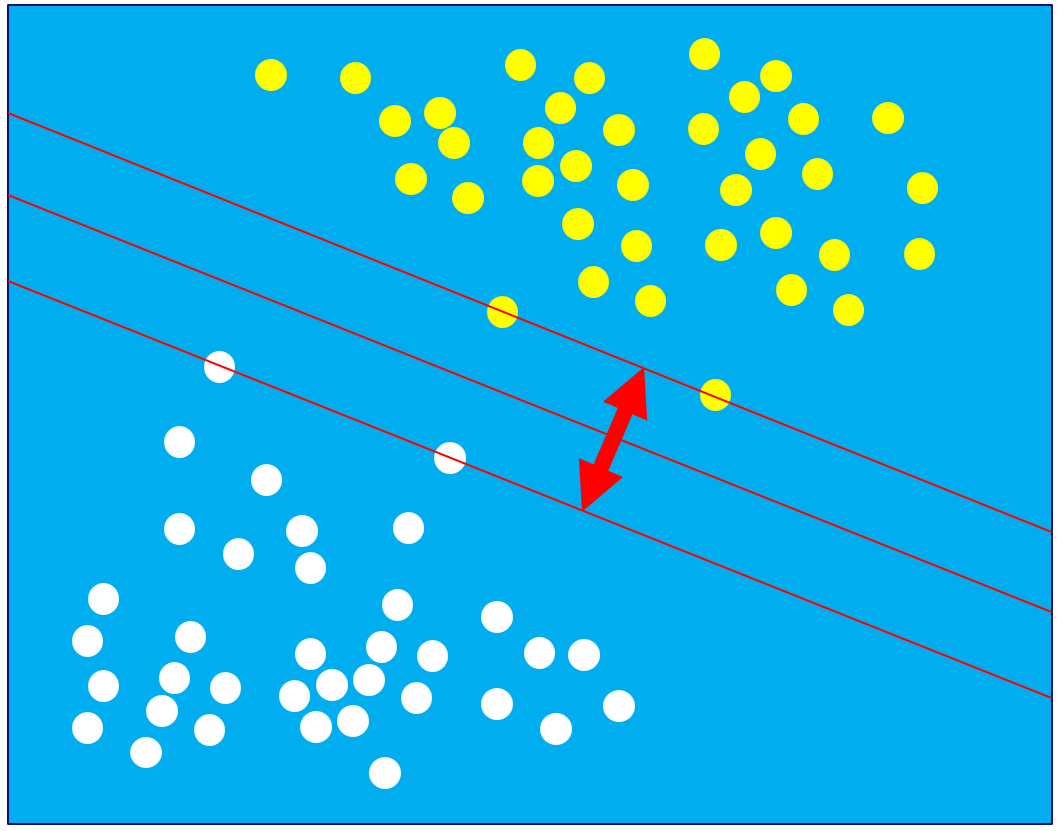
\includegraphics[width=0.55\textwidth]{assets/svm/sm__nice_separation.png}
    \subcaption{Nicely separable data}
  \end{subfigure}\hspace*{0.05\textwidth}
  \begin{subfigure}{0.47\textwidth}
    \centering
    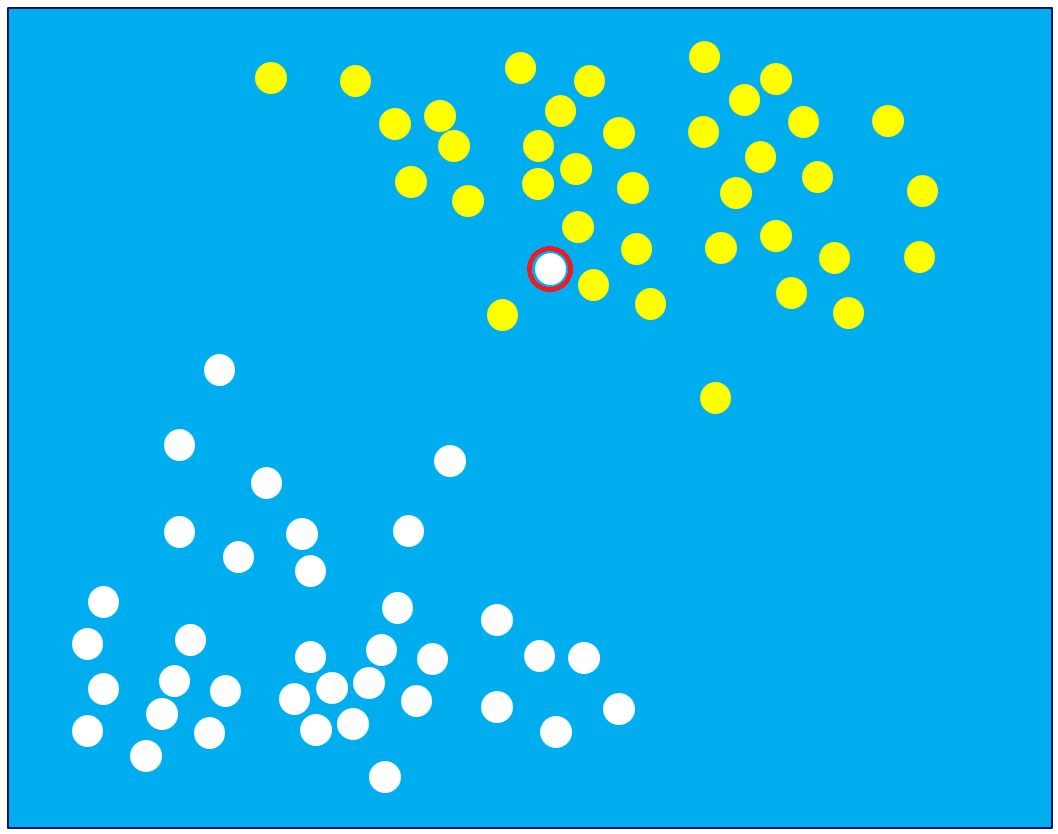
\includegraphics[width=0.55\textwidth]{assets/svm/sm__separation_1_outlier.png}
    \subcaption{One outlier destroying separability}
  \end{subfigure}

  \vspace*{0.3cm}

  
  \begin{subfigure}{0.47\textwidth}
    \centering
    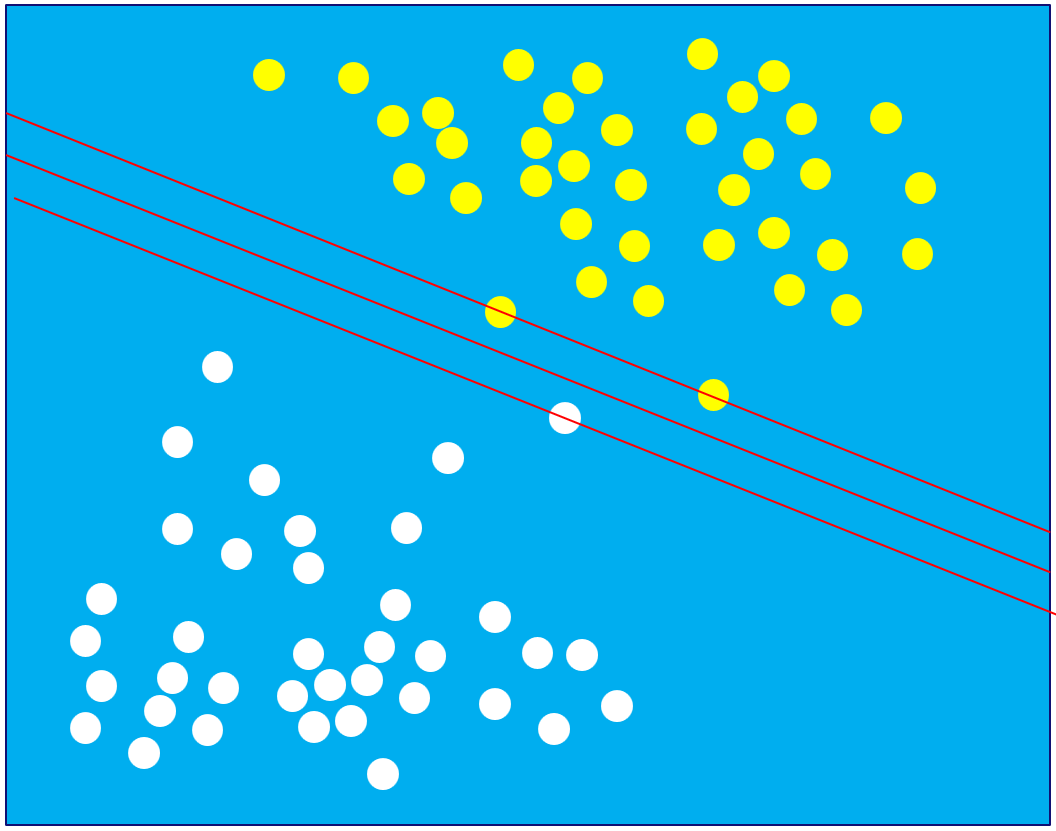
\includegraphics[width=0.55\textwidth]{assets/svm/sm__separation_reduced_margin.png}
    \subcaption{Outlier reducing margin}
    \vspace*{0.5cm}
  \end{subfigure}\hspace*{0.05\textwidth}
  \begin{subfigure}{0.47\textwidth}
    \centering
    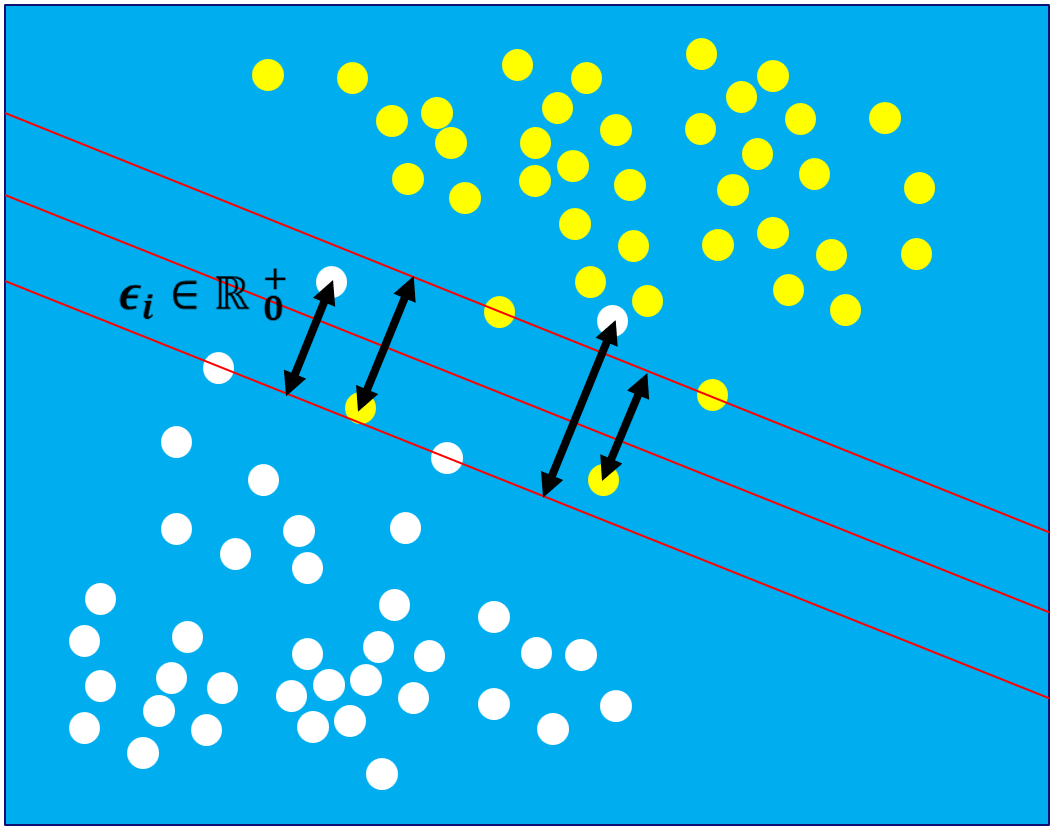
\includegraphics[width=0.55\textwidth]{assets/svm/sm__separation_slack.png}
    \subcaption{Reasonable hyperplane tolerating outliers\\$\rightarrow$ add goal of minimizing slack variables}
  \end{subfigure}

  \caption{Separability of datasets}
  \label{fig:5_not_separable}
\end{figure}

So, the reformulated problem is the following:
\begin{align*}\begin{aligned}
  \text{Given a set of } m \text{ instances }& \big\{ (\cv{x}_i, y_i) \in \mathbb{R}^n\times\{-1,1\} \,\big|\, 1\leq i\leq m \big\}\sidenote{Soft-margin SVM problem}\\
  \min_{\cv{w}, b, {\color{burntorange}\epsilon}}\frac{1}{2}\norm{\cv{w}}^2 {\color{burntorange}+\, C\sum_{i=1}^m\epsilon_i} \text{ s.t. } &\forall i: y_i(\cv{w}\cdot\cv{x}_i + b) \geq 1 {\color{burntorange}-\epsilon_i} \begin{note}\text{ \color{gray}where }\epsilon_i\geq0\end{note}
\end{aligned}\end{align*}

The role of $C$ determines how much we want to restrict tolerance for outliers. 
\begin{itemize}
  \item For a high $C$, we have a strict formulation of our problem, so no outlier tolerance.
  \item For a low $C$, we have a more flexible formulation of the problem, so outliers are tolerated.
  \item Consider \ref{fig:5_c} to see the effect of $C$ on different datasets.
\end{itemize}

\begin{figure}[H]
  \centering
  \begin{subfigure}{\textwidth}
    \centering
    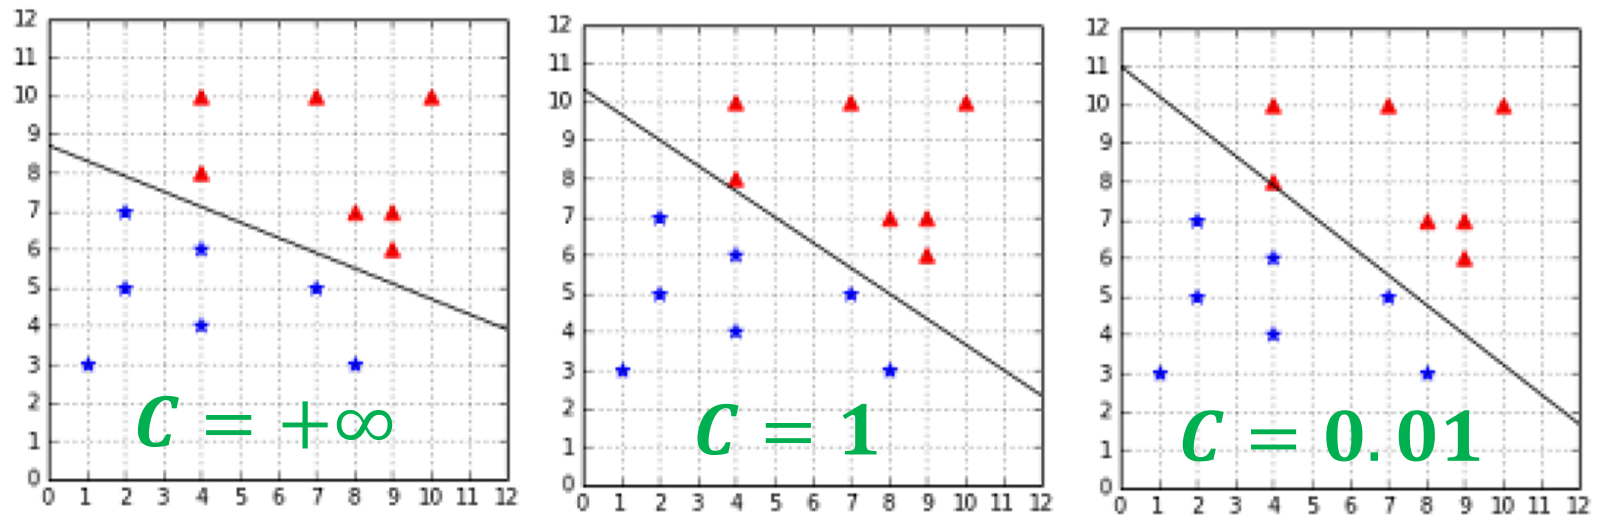
\includegraphics[width=0.6\textwidth]{assets/svm/sm__c_separable.png}
    \subcaption{Separable dataset}
  \end{subfigure}

  \vspace*{0.5cm}

  \begin{subfigure}{\textwidth}
    \centering
    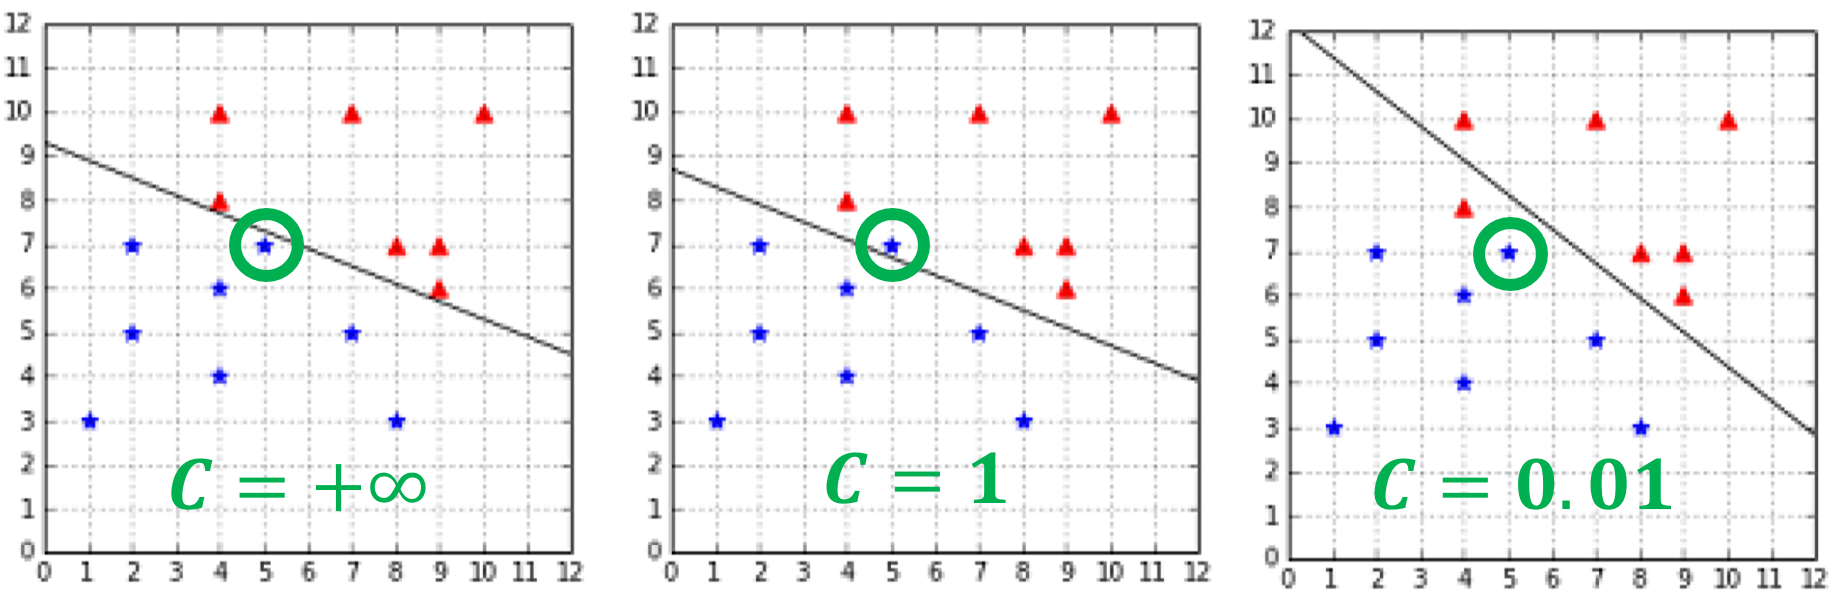
\includegraphics[width=0.6\textwidth]{assets/svm/sm__c_1_outlier.png}
    \subcaption{One outlier, but still separable dataset}
  \end{subfigure}

  \vspace*{0.5cm}

  \begin{subfigure}{\textwidth}
    \centering
    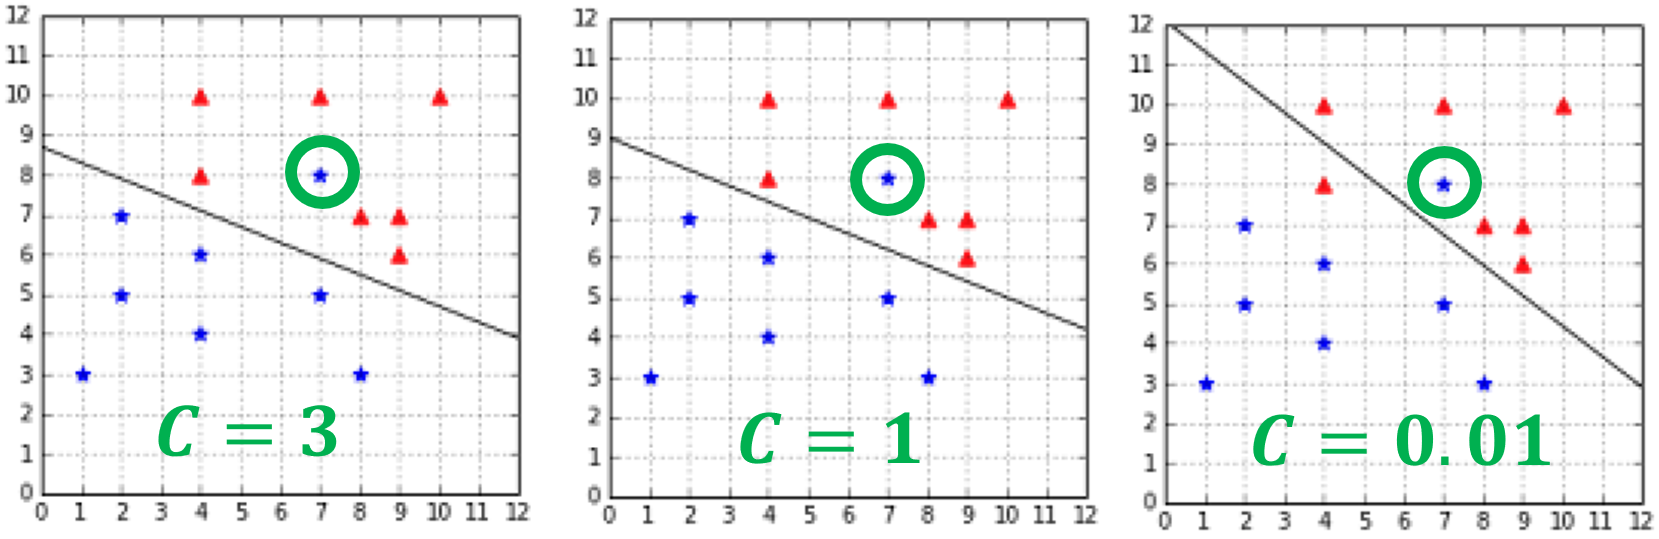
\includegraphics[width=0.6\textwidth]{assets/svm/sm__c_not_separable.png}
    \subcaption{Not separable dataset}
    \text{
      \begin{note}Especially for $C=+\infty$: no solution of SVM exists for this problem\end{note}
    }
  \end{subfigure}

  \caption{Role of $C$ for soft-margin SVM}
  \label{fig:5_c}
\end{figure}